\documentclass[tikz,convert=pdf2svg]{standalone}
\usepackage{tikz}
\begin{document}
    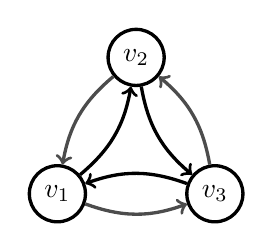
\begin{tikzpicture}
    [L1Node/.style={circle, draw=black, very thick, minimum size=5mm}]
    \node[L1Node] (n1) at (0, 0){$v_1$};
    \node[L1Node] (n2) at (1, 1.732){$v_2$};
    \node[L1Node] (n3) at (2, 0){$v_3$};
    \draw[->, very thick] (n1) to[out=40, in=260] (n2);
    \draw[->, very thick, color=black!70] (n2) to[out=220, in=80] (n1);
    \draw[->, very thick] (n2) to[out=280, in=140] (n3);
    \draw[->, very thick, color=black!70] (n3) to[out=100, in=320] (n2);
    \draw[->, very thick] (n3) to[out=160, in=20] (n1);
    \draw[->, very thick, color=black!70] (n1) to[out=-20, in=200] (n3);
    \end{tikzpicture}
\end{document}